\section{Odnos polova u informatici u svetu}
\interfootnotelinepenalty=10000
\label{sec:usvetu}
Postoji širok konsenzus da su žene manje zastupljeni pol u informatici: prema podacima Eurostata, one čine 18.5\% IKT stručnjaka u Evropskoj Uniji,\cite{gendergap-eu} prema izveštaju britanskog \emph{Tech Nation}-a u Ujedinjenom Kraljevstvu ovaj broj je 19\%,\cite{gendergap-uk} a američki Nacionalni centar za žene i informacionu tehnologiju je 2016. objavio da tek 26\% poslova vezanih za računarstvo obavljaju žene i to prvenstveno na pozicijama projektne menadžerke i biznis analitičarke (dok su muškarci češće softverski inžinjeri i sistem administratori) \cite{gendergap-us}. Još gora situacija je na rukovodećim pozicijama, što se može videti na slici \ref{fig:rukovodece}.

\begin{figure}[h!]
\begin{center}
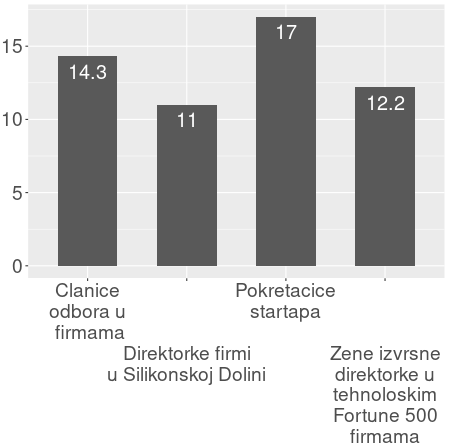
\includegraphics[width=6cm, height=5cm]{zene-na-rukovodecim-pozicijama.png}
\end{center}
\caption{Procenat žena na rukovodećim pozicijama \cite{leadership-women}. Na x osi se nalazi naziv pozicije, a na y procenat žena na toj poziciji.}
\label{fig:rukovodece}
\end{figure}

U ovom odeljku ćemo dati pregled literature s ciljem da čitaoca upoznamo sa položajem žena u informatici i razlozima zašto je on takav. Pošto u literaturi često ne postoje precizniji termini, koristićemo srodne oblasti u prezentaciji podataka i zaključaka. Tako ćemo kada pričamo o Evropi uglavnom posmatrati blisku oblast informacionih i komunikacionih tehnologija (IKT), a u Americi ćemo se češće susretati sa nešto širom grupom već pomenutih MINT oblasti.

\subsection{Obrazovanje i analogija bušne cevi}
Jedno od popularnijih objašnjenja za činjenicu da su žene manje zastupljene u MINT poslovima u odnosu na relevantne obrazovne smerove u preduniverzitetskom i univerzitetkom obrazovanju je preko analogije ,,bušne cevi'': iako je na početnim stupnjevima odnos polova ujednačeniji, učenice i studentkinje neproporcionalno više odustaju na svakom koraku svog obrazovnog puta \cite{jacobs, soe-yakura, blickenstaff}. Međutim, ova analogija nije opšteprihvaćena. Leventman primećuje da postoje tri načina pomoću kojih se može doći do karijere u informatici: tradicionalni, nakon višeg obrazovanja, zatim tranzicioni, ako zaposlena dolazi iz druge oblasti, i samousmereni tj. samouki \cite{leventman}. Ovo znači da osim ,,curenja'' postoji i obrnut proces, ,,ubrizgavanje''. Bartol i Esprej navodne konkretan primer Sjedinjenih država 1996. godine, kada se broj poslova povećao za 200000, a broj dodeljenih diploma u informatičkim disciplinama je bio svega 45000 na svim stepenima studija \cite{bartol}.

So i Jakura analogiju cevi odbacuju kao prejednostavnu, te da umesto traženja rešenja za probleme u jednoj ili par faza u obrazovanju ili zapošljavanju (npr. fokusiranje samo na fakultet ili zapošljavanje), problem treba posmatrati iz dublje kulturološke perspektive. One takođe tvrde da nije dovoljno imati samo nekoliko pojedinaca koji bi rešavali problem ili bili primer, već je neophodno ostvariti kritičnu masu žena i/ili muškaraca, na vodećim pozicijama koji bi razumeli i adekvatno adresirali sve probleme koji dovode do neravnopravnosti na nivou celokupne zajednice \cite{soe-yakura}.

\subsection{Razlozi za nejednaku zastupljenost} 
Postoji nekoliko različitih grupa teorija zašto su žene manje zastupljen pol. Najjednostavnija krivicu pripisuju nedostatku sposobnosti devojčica i žena: Bares ovo naziva ,,hipotezom Lerija Samersa'' po bivšem predseniku Harvarda i opisuje kao krivljenje žrtve \cite{barres}. Samers je jednom prilikom izjavio da su glavni razlozi manje zastupljenosti žena u inženjerskim disciplinama genetske predispozicije i lični izbori; ovo je izazvalo velika negodovanja u naučnoj zajednici i tvrdnje da su njihova istraživanja pogrešno interpretirana, a Samers se kasnije izvinio zbog svojih reči \cite{lawler}.

Druga grupa pretpostavlja da je u pitanju njihov izbor prouzrokovan različitim okolnostima\cite{hellens, blickenstaff}. Blikenstaf odbacuje biološke razlike i nudi jednu sistematizaciju razloga zašto devojčice češće odustaju od karijere u MINT oblastima: u manjoj meri nedostatak pozitivnih iskustava devojčica sa naukom i averzija prema relevantnim predmetima, nedostatak ženskih uzora i neadekvatni kurikulumi, a značajnije neadekvatan pedagoški pristup nastavnika, klima u kojoj se favorizuju i više se očekuje od dečaka i muški pogled na svet koji dominira u nauci \cite{blickenstaff}. Treća grupa objašnjenja se fokusira na prepreke na koje žene nailaze u svom akademskom i karijernom putu: Svaford i kolege kao neke od faktora koji sputavaju žene u MINT karijerama navode seksizam i postojanje ,,staklenog plafona'' za žene u ovim poslovima \cite{swafford}.

Kada je reč o zaposlenju, Vin i Korel su ispitivale kako se predstavnici tehnoloških kompanija odnose prema potencijalnim kandidatima, studentima završnih godina na jednom američkom univerzitetu koji su izrazili interesovanje za poziciju u kompanijama. One su primetile da su već u inicijalnom koraku pri zapošljavanju zastupljene razne prakse koje su diskriminatorne prema ženama. Ističu da je tipično da muškarci dominiraju u vodećim ulogama na intervjuima, dok su žene često marginalizovane ili su zadužene samo za netehničke delove. Takođe su učestale reference na štrebersku (eng. \emph{geek}) kulturu, koja je po prirodi maskulina, kao i propagiranje rodnih stereotipa, što ima veliki potencijal da odbije ženske kandidate u startu. Manje startap firme su posebno odgovorne za deljenje poklona koji mogu biti uvredljivi ženama, poput majici s natpisima \emph{'I like big data and I cannot lie'} (referenca na pesmu \emph{Sir Mix-A-Lot}-a iz 1992), \emph{'I’ll show you my data if you show me yours.'} i \emph{'Finding your faults, just like mom'} \cite{wynn}. Startapi i startap kultura se često karakterišu kao seksističke, a ove firme iako pojedinačno male, čine nezanemarljiv deo poslodavaca \cite{steinberg-forbes}.

U jednom od istraživanja koje se fokusiralo na radnu populaciju, Levelin i kolege su sproveli istraživanje nad alumnijima \emph{Georgia Tech}-a koji su se u međuvremenu zaposlili, s ciljem da saznaju više o karijernim putevima žena i manjinskim grupama u IT sektoru. Jedan od rezultata, koji se fokusira na iskustva na poslu, je da žene značajno češće kažu da su diskriminisane na poslu i da su značajno manje zadovoljne benefitima (obe skale su nastale agregiranjem više relevantnih stavki koje međusobno koreliraju, tj. istraživači prezentovali rezultate kroz kompozitne mere) \cite{llewellyn}.

Evidentna je i razlika u plati, pa tako žene u tehnološkom sektoru u Sjedinjenim Državama primaju u proseku 8600 dolara godišnje manje od njihovih muških kolega, a razlika između polova postoji čak i kada se uzmu u obzir i drugi faktori poput iskustva, pozicije, lokacije i obrazovanja \cite{dhi}. Segovia-Perez i koleginice su analizirale podatke za Španiju i zaključile da ova razlika procentualno raste kako se povećavaju plate, što ukazuje na diskriminaciju prema ženama, posebno na višim pozicijama \cite{segovia}.

Iako smo se do sad fokusirali na Evropu i Ameriku, važno je napomenuti da slična iskustva žena i odnosi između polova u informatici nisu univerzalna. Recimo, u Maleziji su žene dominantan pol na IKT studijama, a iako ne postoji precizna statistika o zastupljenosti polova prema oblasti zaposlenja, postoji razlog da se veruje da žene nisu manje zastupljen pol u IKT ni nakon studija. Melstrom u svom radu izlaže detaljnu analizu ove pojave i sagledava rodne, ali i istorijske, etničke i kulturološke specifičnosti Malezije i konkretne intervencije u informatičkom obrazovanju i predlaže sličan pristup za druge države  \cite{mellstrom}. Zaključci iz ovog istraživanja se teško mogu generalizovati, ali nas podsećaju da je drugačija realnost moguća kao rezultat pažljivo odabranih intervencija i politika.

Još jedna zanimljiva pojava je paradoks jednakosti polova u MINT oblastima: Stoet i Giri su pronašli direktnu korelaciju između rodne egalitarnosti i manje zastupljenosti žena na MINT studijama, suprotno od onoga što je intuitivno očekivano \cite{stoet}. Međutim, ovo istraživanje je postalo kontroverzno kada Ričardson i kolege\cite{richardson} nisu uspeli da reprodukuju ove rezultate, a ni u ispravci originalnog nisu promenjeni zaključi. Ova rasprava nije dobila epilog i ne postoji širi naučni konsenzus o ovome \cite{schleunes-scientist}.
\subsection{Razlika između akademije i industrije}
Zastupljenost istraživačica u tehnološkim i inženjerskim oblastima u višem obrazovanju u Evropi varira, od 14.94\% u Luksemburgu i 15.73\% na Malti, do 39.3\% u Crnoj Gori i 44.4\% u Rumuniji, prema podacima Evropske Unije za 2017. godinu \cite{shefigures}. S obzirom da nisu sve zemlje učestvovale u ovom istraživanju svake godine, teško je doći do verodostojne vrednosti proseka, ali je bezbedno reći da je on nešto povoljniji za žene nego zbirne brojke date na početku ovog poglavlja.\footnote{Zainteresovani čitalac može pronaći podatke u interaktivnom obliku na portalu Evropske kancelarije za publikacije na adresi \url{https://quantos-stat.shinyapps.io/GUI_SF/}. U meniju s leve strane odabrati \emph{Chapter 4}, indikator \emph{Proportion (\%) of women among researchers}, jedinicu \emph{HC} (headcount), sektor \emph{HES} (higher education) i polje \emph{Engineering and technology}.} S obzirom na ovoliki raspon, nije moguće generalizovati bilo koji konkretan zaključak na ceo kontinent, posebno pošto postoje države u kojima je situacija skoro ravnopravna.

U Sjedinjenim Američkim Državama, situacija je obrnuta: u akademiji se računarskim naukama bavi svega 15\% žena \cite{way}. Neke od razloga zašto je razlika u polovima ovde veća možemo potražiti u činjenici da je razlika u plati izraženija u akademiji (i to za 50\% u odnosu na industriju, prema istraživanju koje su sproveli Ding i kolege \cite{ding}) i da je akademska karijera dosta nepovoljnija po (buduće) majke, s obzirom da su u SAD trudnički i porodiljski benefiti (uključujući i karijerni put novih roditelja) bolji u industriji \cite{morgan}. Ovi razlozi u opštem slučaju ne važe za Evropu.